\documentclass[journal,12pt,twocolumn]{IEEEtran}

\usepackage{setspace}
\usepackage{paralist}
\usepackage{gensymb}
\singlespacing
\usepackage[cmex10]{amsmath}

\usepackage{amsthm}
\usepackage{amssymb}

\usepackage{mathrsfs}
\usepackage{txfonts}
\usepackage{stfloats}
\usepackage{bm}
\usepackage{cite}
\usepackage{cases}
\usepackage{subfig}

\usepackage{longtable}
\usepackage{multirow}

\usepackage{enumitem}
\usepackage{mathtools}
\usepackage{steinmetz}
\usepackage{tikz}
\usepackage{circuitikz}
\usepackage{verbatim}
\usepackage{tfrupee}
\usepackage[breaklinks=true]{hyperref}
\usepackage{graphicx}
\usepackage{tkz-euclide}

\usetikzlibrary{calc,math}
\usepackage{listings}
    \usepackage{color}                                            %%
    \usepackage{array}                                            %%
    \usepackage{longtable}                                        %%
    \usepackage{calc}                                             %%
    \usepackage{multirow}                                         %%
    \usepackage{hhline}                                           %%
    \usepackage{ifthen}                                           %%
    \usepackage{lscape}     
\usepackage{multicol}
\usepackage{chngcntr}
\usepackage{mathtools}
\DeclarePairedDelimiter\ceil{\lceil}{\rceil}
\DeclarePairedDelimiter\floor{\lfloor}{\rfloor}

\DeclareMathOperator*{\Res}{Res}

\renewcommand\thesection{\arabic{section}}
\renewcommand\thesubsection{\thesection.\arabic{subsection}}
\renewcommand\thesubsubsection{\thesubsection.\arabic{subsubsection}}

\renewcommand\thesectiondis{\arabic{section}}
\renewcommand\thesubsectiondis{\thesectiondis.\arabic{subsection}}
\renewcommand\thesubsubsectiondis{\thesubsectiondis.\arabic{subsubsection}}


\hyphenation{op-tical net-works semi-conduc-tor}
\def\inputGnumericTable{}                                 %%

\lstset{
%language=C,
frame=single, 
breaklines=true,
columns=fullflexible
}
\begin{document}

\newcommand{\BEQA}{\begin{eqnarray}}
\newcommand{\EEQA}{\end{eqnarray}}
\newcommand{\define}{\stackrel{\triangle}{=}}
\bibliographystyle{IEEEtran}
\raggedbottom
\setlength{\parindent}{0pt}
\providecommand{\mbf}{\mathbf}
\providecommand{\pr}[1]{\ensuremath{\Pr\left(#1\right)}}
\providecommand{\qfunc}[1]{\ensuremath{Q\left(#1\right)}}
\providecommand{\sbrak}[1]{\ensuremath{{}\left[#1\right]}}
\providecommand{\lsbrak}[1]{\ensuremath{{}\left[#1\right.}}
\providecommand{\rsbrak}[1]{\ensuremath{{}\left.#1\right]}}
\providecommand{\brak}[1]{\ensuremath{\left(#1\right)}}
\providecommand{\lbrak}[1]{\ensuremath{\left(#1\right.}}
\providecommand{\rbrak}[1]{\ensuremath{\left.#1\right)}}
\providecommand{\cbrak}[1]{\ensuremath{\left\{#1\right\}}}
\providecommand{\lcbrak}[1]{\ensuremath{\left\{#1\right.}}
\providecommand{\rcbrak}[1]{\ensuremath{\left.#1\right\}}}
\theoremstyle{remark}
\newtheorem{rem}{Remark}
\newcommand{\sgn}{\mathop{\mathrm{sgn}}}
\providecommand{\abs}[1]{\vert#1\vert}
\providecommand{\res}[1]{\Res\displaylimits_{#1}} 
\providecommand{\norm}[1]{\lVert#1\rVert}
%\providecommand{\norm}[1]{\lVert#1\rVert}
\providecommand{\mtx}[1]{\mathbf{#1}}
\providecommand{\mean}[1]{E[ #1 ]}
\providecommand{\fourier}{\overset{\mathcal{F}}{ \rightleftharpoons}}
%\providecommand{\hilbert}{\overset{\mathcal{H}}{ \rightleftharpoons}}
\providecommand{\system}{\overset{\mathcal{H}}{ \longleftrightarrow}}
	%\newcommand{\solution}[2]{\textbf{Solution:}{#1}}
\newcommand{\solution}{\noindent \textbf{Solution: }}
\newcommand{\cosec}{\,\text{cosec}\,}
\providecommand{\dec}[2]{\ensuremath{\overset{#1}{\underset{#2}{\gtrless}}}}
\newcommand{\myvec}[1]{\ensuremath{\begin{pmatrix}#1\end{pmatrix}}}
\newcommand{\mydet}[1]{\ensuremath{\begin{vmatrix}#1\end{vmatrix}}}
\numberwithin{equation}{subsection}
\makeatletter
\@addtoreset{figure}{problem}
\makeatother
\let\StandardTheFigure\thefigure
\let\vec\mathbf
\renewcommand{\thefigure}{\theproblem}
\def\putbox#1#2#3{\makebox[0in][l]{\makebox[#1][l]{}\raisebox{\baselineskip}[0in][0in]{\raisebox{#2}[0in][0in]{#3}}}}
     \def\rightbox#1{\makebox[0in][r]{#1}}
     \def\centbox#1{\makebox[0in]{#1}}
     \def\topbox#1{\raisebox{-\baselineskip}[0in][0in]{#1}}
     \def\midbox#1{\raisebox{-0.5\baselineskip}[0in][0in]{#1}}
\vspace{3cm}
\title{\textbf{AI1103 : Assignment 4}}
\author{\textbf{Santosh Dhaladhuli MS20BTECH11007}}
\maketitle
\newpage
\bigskip
\renewcommand{\thefigure}{\theenumi}
\renewcommand{\thetable}{\theenumi}

Download all python codes from 
\begin{lstlisting}
https://github.com/Santosh-Dhaladhuli2003/AI1103/blob/main/Assignment%202/Assignment%202.py
\end{lstlisting}
%
and latex codes from 
%
\begin{lstlisting}
https://github.com/Santosh-Dhaladhuli2003/AI1103/blob/main/Assignment%202/Assignment%202.tex
\end{lstlisting}
\section{\textbf{GATE CS 2015 Set-1 Question No. 10}}
The probabilities that a student passes in Mathematics, Physics and Chemistry are m, p and c respectively.Of these subjects,the student has 75$\%$ chance of passing in at least one,a 50$\%$ chance of passing in at least two and a 40$\%$ chance of passing in exactly two. Following relations are drawn in m, p and c:
 \begin{enumerate}[label=(\roman*)]
 \item p + m + c = $\frac{27}{20}$ 
 \item p + m + c = $\frac{13}{20}$ 
 \item p $\times$ m $\times$ c = $\frac{1}{10}$
 \end{enumerate}
 \vspace{0.5cm}
\begin{enumerate}
    \item Only relation (i) is true
    \item Only relation (ii) is true
    \item Relations (ii) and (iii) are true
    \item Relations (i) and (iii) are true
\end{enumerate}

\section{\textbf{Solution}}
Let X be a Random variable that denotes number of subjects the student passes. \\
So, X $\in$ {0,1,2,3} \\
Given,
\begin{table}[h]
\begin{tabular}{|l|l|}
\hline
P(X $\ge$ 1) & 0.75 \\ \hline
P(X $\ge$ 2) & 0.50 \\ \hline
P(X = 2)   & 0.40 \\ \hline
\end{tabular}
\end{table}
\begin{equation}
\tag{1.1}
\pr{X = 0}  = 1 - \pr{X \ge 1} = 1 - 0.75 \label{1} 
\end{equation}
\begin{equation}
    \tag{1.2}
\implies \pr{X = 0} = 0.25= \text{(1 - m)(1 - p)(1 - c)}
\end{equation}
\begin{equation}
    \tag{1.3}
    \implies \text{m + p + c  + mpc - mp - cm -pc} = 0.75 \label{X = 0}
\end{equation}
\begin{equation}
    \tag{1.4}
\pr{X = 2} = \text{mp(1 - c)+ pc(1- m)+ cm(1 - p)} = 0.40
\end{equation}
\begin{equation}
\tag{1.5}
    \implies \text{mp + pc + cm - 3mpc} = 0.4 \label{X = 2}
\end{equation}
\begin{equation}
    \tag{1.6}
    \pr{X \ge 2} = \pr{X = 2} + \pr{X = 3} = 0.5 
\end{equation}
\begin{equation}
\tag{1.7}
    \implies \pr{X = 3} = \text{pmc} = 0.1 = \frac{1}{10} \label{X = 3}
\end{equation}
\vspace{0.1cm}
$\therefore$ \textbf{Relation (iii) is TRUE}

Substituting \eqref{X = 3} in \eqref{X = 2},
\begin{equation}
    \tag{1.8}
    \implies \text{mp + cm + pc} = 0.7 \label{a}
\end{equation}
and substituting \eqref{a} and \eqref{X = 3} in \eqref{X = 0}
\begin{equation}
    \tag{1.9}
    \implies \text{m + p + c} = 1.35 = \frac{27}{20}
\end{equation}
$\therefore$ \textbf{Relation (i) is TRUE} \\
From this, the final answer we get is \textbf{Option 4}
\begin{figure}[!htb]
\centering
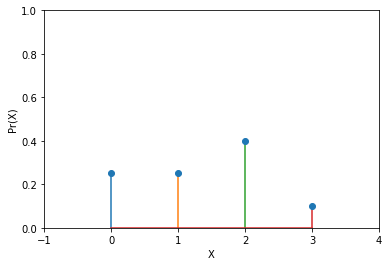
\includegraphics[width=0.45\textwidth]{Assignment 4.png}
\caption{Probability(P(X)) of passing X subjects}
\end{figure}
\end{document}
